\documentclass[12pt]{article}
\usepackage[margin=2.5cm]{geometry}
\usepackage{enumerate}
\usepackage{amsfonts}
\usepackage{amsmath}
\usepackage{fancyhdr}
\usepackage{amsmath}
\usepackage{amssymb}
\usepackage{amsthm}
\usepackage{mdframed}
\usepackage{graphicx}
\usepackage{subcaption}
\usepackage{adjustbox}
\usepackage{listings}
\usepackage{xcolor}
\usepackage{courier}
\usepackage[utf]{kotex}
\usepackage{hyperref}
\usepackage{soul}

\definecolor{codegreen}{rgb}{0,0.6,0}
\definecolor{codegray}{rgb}{0.5,0.5,0.5}
\definecolor{codepurple}{rgb}{0.58,0,0.82}
\definecolor{backcolour}{rgb}{0.95,0.95,0.92}

\lstdefinestyle{mystyle}{
    backgroundcolor=\color{backcolour},
    commentstyle=\color{codegreen},
    keywordstyle=\color{magenta},
    numberstyle=\tiny\color{codegray},
    stringstyle=\color{codepurple},
    basicstyle=\ttfamily\footnotesize,
    breakatwhitespace=false,
    breaklines=true,
    captionpos=b,
    keepspaces=true,
    numbers=left,
    numbersep=5pt,
    showspaces=false,
    showstringspaces=false,
    showtabs=false,
    tabsize=1
}

\lstset{style=mystyle}

\pagestyle{fancy}
\renewcommand{\headrulewidth}{0.4pt}
\lhead{CSC 369}
\rhead{Midterm 3 Notes}

\begin{document}
\title{CSC 369 Midterm 3 Notes}

\section{Virtualizing CPU}

\begin{itemize}
    \item Turns a single CPU into a seemingly infinite number of CPUS, and
    allows many programs to seemingly run at once
    \item To implement CPU virtualization, the OS needs low-level machinery
    called \textbf{mechanism} and high level intelligence called \textbf{policies}
    \item Steps

    \begin{enumerate}[1.]
        \item Involve OS to setup hardware hardwre to limit what the process can do without OS assistance
        (\textbf{Limited Direct Execution})

        \bigskip

        This is done so by

        \bigskip

        \begin{enumerate}[1.]
            \item Setting up trap handler
            \item Starting an interrupt timer (so process won't last forever)
        \end{enumerate}
        \item Involve OS to intervene at key points to perform previleged operations
        or switch out operations when they have monopolized the CPU too long
    \end{enumerate}
    \bigskip
\end{itemize}

\section{Limited Direct Execution}

\begin{itemize}
    \item Idea: Just run the program you want to run on the CPU,
    but first make sure to set up the hardware so as to limit what
    process can do without OS assistance
    \item baby proofs the CPU by

    \bigskip

    \begin{enumerate}[1.]
        \item Setting up trap handlers
        \item Starts an interrupt timer
        \item Run processes in a restricted mode
    \end{enumerate}

    \bigskip

    \underline{\textbf{Example}}

    \bigskip

    Baby proofing a room:

    \bigskip

    \begin{itemize}
        \item Locking cabinets containing dangerous stuff and covering electrical sockets.
        \item When room is readied, let your baby roam free in knowledge that all the dangerous
        aspect of the room is restricted
    \end{itemize}
\end{itemize}

\section{Trap Handlers}

\begin{itemize}
    \item Is instruction that tells the hardware what to run when certain exceptions occur

    \bigskip

    \underline{\textbf{Example}}

    \bigskip

    What code to run when

    \begin{enumerate}[1.]
        \item Hard disk interrupt occurs
        \item Keyboard interrupt occrs
        \item Program makes a system call?
    \end{enumerate}

\end{itemize}

\section{Timer Interrupt}

\begin{itemize}
    \item Is a hardware mechanism that ensures the user program does not run forever
    \item Is emitted at regular intervals by a timer chip $^{[6]}$
\end{itemize}

\section{Response Time}
\begin{itemize}
    \item \textbf{Formula} $T_{response} = T_{firstrun} - T_{arrival}$
    \item measures the interactive performance between users and the system
\end{itemize}

\section{Turnaround Time}

\begin{itemize}
    \item \textbf{Formula} $T_{turnaround} = T_{completion} - T_{arrival}$
    \item measures the amount of time taken to complete a process
\end{itemize}

\section{Starvation}

\begin{itemize}
    \item Is the problem that occurs when high priority processes keep
    executing and low priority processes get blocked for indefinite time $^{[1]}$
\end{itemize}

\section{Convoy Effect}

\begin{itemize}
    \item Is the problem where number of relatively-short potential consumers
    of a resource get queued behind a heavy weight consumer

    \bigskip

    \begin{center}
    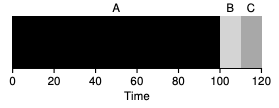
\includegraphics[width=0.7\linewidth]{../images/midterm_2_solution_5.png}
    \end{center}
\end{itemize}

\section{Scheduling policies}

\begin{itemize}
    \item Are algorithms for allocating CPU resources to concurrent tasks
    deployed on (i.e., allocated to) a processor (i.e., computing resource)
    or a shared pool of processors $^{[5]}$
    \item Are sometimes called \textbf{Discipline}
    \item Covers the following algorithms in textbook

    \begin{itemize}
        \item \textbf{First In First Out}

        \begin{itemize}
            \item Is the most basic scheduling algorithm
            \item Is vulnerable to \textbf{convoy effect}
            \item No \textbf{starvation} as long as every process eventually completes
        \end{itemize}

        \item \textbf{Shortest Job First}

        \begin{itemize}
            \item Improves average \textbf{turnaround time} given processes of uneven length
            \item Is a general scheduling principle useful in situation where turnaround time
            per process matters
            \item Is vulnerable to \textbf{convoy effect}

            \begin{center}
            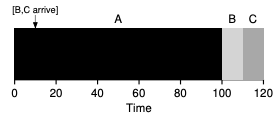
\includegraphics[width=0.7\linewidth]{../images/midterm_2_solution_6.png}
            \end{center}

            \item Is vulnerable to \textbf{starvation}
            \begin{itemize}
                \item When only short-term jobs come in while a long term job is in queue
            \end{itemize}
        \end{itemize}
        \item \textbf{Shortest Time-to-completion First}

        \begin{itemize}
            \item Addresses \textbf{convoy effect} in \textbf{Shortest Job First}
            \item Determines which of the remaining+new jobs has least time left, and
            schedule accordingly at \underline{any time}

            \bigskip

            \begin{center}
            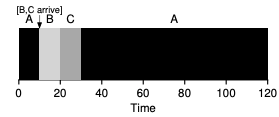
\includegraphics[width=0.7\linewidth]{../images/midterm_2_solution_7.png}
            \end{center}

            \item Is vulnerable to \textbf{starvation}
            \begin{itemize}
                \item When only short-term jobs come in while a long term job is in queue
            \end{itemize}

        \end{itemize}

        \item \textbf{Round Robin}

        \begin{itemize}
            \item Has good \textbf{response time} but terrible \textbf{turnaround time}
            \item Runs job for a \textbf{time slice} or \textbf{quantum}
            \item Each job gets equal share of CPU time
            \item Is clock-driven $^{[6]}$
            \item Is starvation-free $^{[7]}$
            \item \underline{Must} have the length of a time slice (\textbf{quantum}) as multiple of timer-interrupt period
        \end{itemize}

        \bigskip

        \begin{center}
        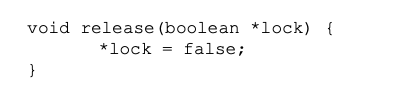
\includegraphics[width=0.7\linewidth]{../images/midterm_2_solution_4.png}
        \end{center}
        \item \textbf{Multi-level Feedback Queue}

        \begin{itemize}
            \item Is the most well known approaches to shceduling
            \item Optimizes \textbf{turnaround time}, and minimizes \textbf{response time}
            \item Observees the execution of a job and priortizes accordingly without prior knowledge
            \item Rules

            \begin{itemize}
                \item \textbf{Rule 1:} If Priority(A) $>$ Priority(B), A runs (B doesn't)
                \item \textbf{Rule 2:} If Priority(A) $=$ Priority(B). A \& B run in round-robin
                fashion using the time slice (quantum length) of the given queue
                \item \textbf{Rule 3:} When a job enters the system, it is placed at the highest
                priority(the top most queue)
                \item \textbf{Rule 4:} Once a job uses up its time allotment at a given level
                (regardless of how many times it has given up the CPU), its priority is reduced
                (it moves down on queue)
                \item \textbf{Rule 5:} After some time period S, move all the jobs in the system to the
                topmost queue.
            \end{itemize}

            \bigskip

            \begin{center}
            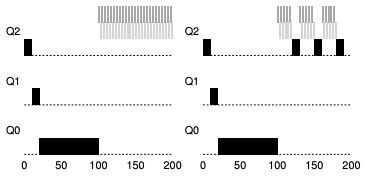
\includegraphics[width=0.7\linewidth]{../images/midterm_2_solution_8.png}
            \end{center}
        \end{itemize}
    \end{itemize}
\end{itemize}

\section{User Mode}

\begin{itemize}
    \item Is restricted
    \item Executing code has no ability to \textit{directly} access
    hardware or reference memory $^{[1]}$
    \item Crashes are always recoverable $^{[1]}$
    \item Is where most of the code on our computer / applications are executed $^{[3]}$
\end{itemize}

\section{Kernel Mode}
\begin{itemize}
    \item Is previleged (non-restricted)
    \item Executing code has complete and unrestricted access to the underlying hardware $^{[3]}$
    \item Is generally reserved for the lowest-level, most trusted functions of the operating
    system $^{[1]}$
    \item Is fatal to crash; it will halt the entire PC (i.e the blue screen of death) $^{[3]}$
\end{itemize}

\section{Interrupt}

\begin{itemize}
    \item i is a signals are sent by hardware (keyboardm mouse, etc.), or software (page fault, protection violation, system call)
    \item Tells the CPU to stop its current activities and execute the appropriate part of the operating system (\textbf{Interrupt Handler}). $^{[2]}$
    \item Has three different types $^{[2]}$

    \begin{enumerate}[1)]
        \item \textbf{Hardware Interupts}

        \begin{itemize}
            \item Are generated by hardware devices to signal that they need some attention from the OS.
            \item May be due to receiving some data

            \bigskip

            \underline{\textbf{Examples}}

            \bigskip

            \begin{itemize}
                \item Keystrokes on the keyboard
                \item Receiving data on the ethernet card
            \end{itemize}

            \bigskip

            \item May be due to completing a task which the operating system previous requested

            \bigskip

            \underline{\textbf{Examples}}

            \bigskip

            Transfering data between the hard drive and memory
        \end{itemize}

        \bigskip

        \item \textbf{Software Interupts}

        \bigskip

        \begin{itemize}
            \item Are generated by programs when a system call is requested
        \end{itemize}

        \bigskip

        \item \textbf{Traps}

        \bigskip

        \begin{itemize}
            \item Are generated by the CPU itself
            \item Indicate that some error or condition occured for which assistance from the operating system is needed
        \end{itemize}

        \bigskip
    \end{enumerate}
\end{itemize}

\section{Trap}
\begin{itemize}
    \item Is an exception in a user process $^{[1]}$
    \item Is an interrupt caused by an exceptional condition (breakpoint, division by zero, invalid memory access) $^{[2]}$
    \item Is called by user
    \item Usually results in kernel mode by invoking \textbf{trap instruction}$^{[2]}$
\end{itemize}

\section{Trap Instruction}

\begin{itemize}
    \item when \textbf{Trap} or \textbf{System call} is invoked, \textbf{Trap instruction}
    simultaneously jumps into the kernel and raise the previlege
    level to kernel mode
\end{itemize}

\section{Context Switch}

\begin{itemize}
    \item Is switching from running a user level process to the OS kernel and often
    to other user processes before the current process is resumed
    \item Happens during a timer interrupt or system call
    \item Saves the following states for a process during a context switch
    \begin{itemize}
        \item Stack Pointer
        \item Program Counter
        \item User Registers
        \item Kernel State
    \end{itemize}
    \item May hinder performance
\end{itemize}

\section{System Call}

\bigskip

\begin{itemize}
    \item Is the programmatic way in which a computer program requests a previleged service from the kernel of the operating system
    \item i.e. Reading from disk
    \item \underline{traps} into the kernel so that priviliged instruction can be run
    \item Provides services via API or Application Program Interface
    \item Is the only entry points into the kernel system
    \item Is strictly a subset of software interrupts
    \item Steps

    \begin{enumerate}[1)]
        \item Setup \textbf{trap tables} on boot
        \item Execute system call
        \item Save \textit{Program Counter}, \textit{CPU registers}, \textit{kernal stack} (so process can resume after \textbf{return-from-trap}
        or \textbf{context switch})
        \item Switch from \textbf{user mode} to \textbf{kernel mode}
        \item Perform previleged operations
        \item Finish and execute \textbf{return-from-trap} instruction
        \item Return from \textbf{kernel mode} to \textbf{user mode} and resume user program
    \end{enumerate}

    \item Has five different types

    \begin{center}
    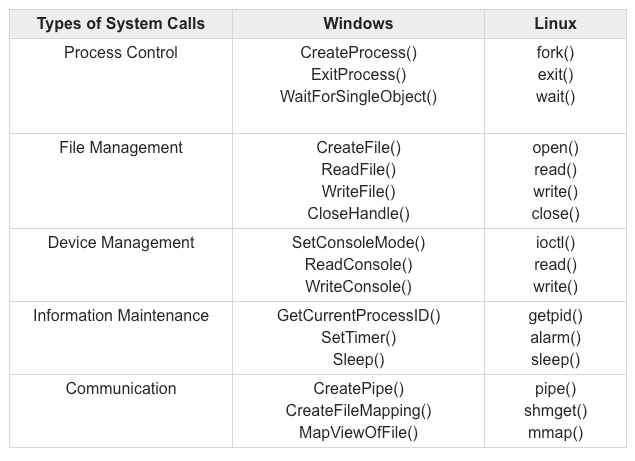
\includegraphics[width=0.7\linewidth]{../images/midterm_3_solution_1.png}
    \end{center}
\end{itemize}

\underline{\textbf{Example}}

\begin{itemize}
    \item \texttt{yield()}
    \begin{itemize}
        \item Is a system call
        \item Causes the calling thread to relinquish the CPU
        \item Places the current thread at the end of the run queue
        \item Schedules another thread to run
    \end{itemize}
\end{itemize}

\bigskip

\underline{\textbf{Example}}

\bigskip

\texttt{open()}, \texttt{read()}, \texttt{write()}, \texttt{close()}, \texttt{mkdir()} are other examples of system calls

\section{Signals}

\begin{itemize}
    \item Provides a way to communicate with the process
    \item Can cause job to stop, continue, or terminate
    \item Can be delivered to an application

    \begin{itemize}
        \item Stops the application from whatever its doing
        \item Runs Signal handler (some code in application to handle the signal)
        \item When finished, the process resumes previous behavior
    \end{itemize}
\end{itemize}

\section{CPU-bound process} $^{[8]}$

\begin{itemize}
    \item CPU Bound processes are ones that are implementing algorithms
    with a large number of calculations
    \item Programs such as simulations may be CPU bound for most of the life of the process.
    \item Users do not typically expect an immediate response from the computer when running CPU bound programs.
    \item They should be given a lower priority by the scheduler.
\end{itemize}
\section{I/O-bound process} $^{[8]}$

\begin{itemize}
    \item Processes that are mostly waiting for the completion of input or output (I/O) are I/O Bound.
    \item Interactive processes, such as office applications are mostly I/O bound the entire life of the process. Some processes may be I/O bound for only a few short periods of time.
    \item The expected short run time of I/O bound processes means that they will not stay the running the process for very long.
    \item They should be given high priority by the scheduler.
\end{itemize}

\section{Memory API}

\begin{itemize}
    \item Has two types of memory

    \begin{enumerate}[1.]
        \item \textbf{Stack}

        \begin{itemize}
            \item Is also called \textbf{automatic memory}
            \item Allocations and deallocations are managed by compiler
            \item Deallocates memory by the end of function call
        \end{itemize}

        \item \textbf{Heap}

        \begin{itemize}
            \item Is long-lived
            \item Allocation and deallocation are managed by user
            \item Creates \textbf{memory leak} if memory not freed
            \item \textbf{valgrind} is a useful heap memoery debugging tool \href{https://www.valgrind.org/docs/manual/quick-start.html}{link}
        \end{itemize}
    \end{enumerate}

    \item \texttt{malloc()}
    \begin{itemize}
        \item Is a C library call
        \item \textbf{Syntax:} \texttt{void *malloc(size\_t size)}
        \item Allocates a block of \texttt{size} bytes to \textbf{heap memory}
        and if successful, returns a pointer to it
        \item Returns \texttt{NULL} if memory allocation is unsuccessful
    \end{itemize}

    \bigskip

    \underline{\textbf{Example}}

    \bigskip

    \texttt{int *x = malloc(10 * sizeof(int));}

    \bigskip
    \item \texttt{free()}
    \begin{itemize}
        \item Is a C library call
        \item Frees heap memory that is no longer in use
    \end{itemize}

    \bigskip

    \underline{\textbf{Example}}

    \bigskip

    \texttt{int *x = malloc(10 * sizeof(int));}\\
    \texttt{...}\\
    \texttt{free(x);}

    \bigskip

    \item \texttt{brk(), sbrk(), mmap()}

    \begin{itemize}
        \item Are system calls for memory management
    \end{itemize}

\end{itemize}

\section{Buffer overflow}
\begin{itemize}
    \item is an error that occurs when not enough heap memory is allocated

    \bigskip

    \begin{center}
    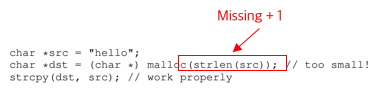
\includegraphics[width=0.8\linewidth]{../images/midterm_3_solution_2.png}
    \end{center}
\end{itemize}

\section{Virtualizing Memory}
\begin{itemize}
    \item Basic Idea: For the most part, let the program run directly on the hardware;
    however, at certain key points in time (e.g. system call, timer interrupt), arrange
    so that the OS gets involved and make sure the 'Right' thing happens.
    \item Like CPU, many programs are sharing the memory at the same time
    \item Like CPU, the goal is to create an illusion that it has its own code and data
    \item Like CPU, the memory also needs low-level machinery called \textbf{mechanism},
    and high level intelligence called \textbf{policies}
    \item Steps

    \begin{enumerate}[1.]
        \item Use \textbf{address translation} to transform each memory access,
        changing \textbf{virtual address} provided by instruction to \textbf{physical address}
        \begin{itemize}
            \item Memory access includes instruction fetch, load, or store
            \item Is done using hardware
        \end{itemize}
        \item Invove OS at key points to \textbf{manage memory}

        \bigskip

        Memory management includes

        \bigskip

        \begin{enumerate}[1.]
            \item Setting up hardware so correct translations take place
            \item Keeping track of which locations are free and which are in use
            \item Judiciously intervening to maintain control over how memory is used
        \end{enumerate}

        \bigskip
    \end{enumerate}
\end{itemize}

\section{Address Translation}

\begin{itemize}
    \item Is also called \textbf{hardware-based address translation}
    \item Is a mechanism of memory virtualization
    \item Is the technique of transforming virtual address to physical address
\end{itemize}

\end{document}